\chapter{Accelerator Physics of Linear Colliders}
\label{LinearColliderPhysics}

\begin{chapterabstract}
Since the invention of the first particle accelerator in 1930, many new forms of accelerators were discovered and developed over the years. 
Even though they may differ in shape and form, they all rely on the same principles. 
After a brief introduction of these principles of accelerator physics, there will be a description of the two classes of particle accelerators which are mainly used for high-energy physics nowadays: linear and circular colliders. 
By looking at their advantages and disadvantages, the differences between them will be elaborated.
\end{chapterabstract}
\newline

In 1930, J. D. Cockcroft and E. T. S. Walton constructed the first particle accelerator, in order to probe the nuclei of lithium atoms with protons accelerated to several hundred keV. 
They found that the key in particle acceleration lies in electrostatics.

\section{Principles of particle acceleration}
\label{AccPhysics:Principles}
Charged particles are accelerated inside an electric field. 
In a time independent electric field $\vec{E}$ with potential $U$, the particle with charge $q$ experiences a change in its kinetic energy by passing through this electric field.
\begin{equation}
 \Delta E = q \int \vec{E}d\vec{r} = qU
\end{equation}
The particle's charge expressed in the elementary charge e is simply multiplied by the electric potential in Volts to calculate the gain or loss of the particle's kinetic energy. 
Out of convenience, the unit for energy in particle physics is therefore eV.\\
By this logic a particle is accelerated to higher energies by applying higher and higher electrostatic fields. 
Exactly this was done in the beginning of particle accelerators by increasing the voltage applied to a capacitor and shooting the charged particle through. 
Unfortunately, there are limits to the amount of voltage that can be applied before an electric breakdown.
The solution seems simple by putting several capacitors in a row.
But again, this can not be done with electrostatic capacitors since the field gradient between two different capacitors is directed in the opposite direction.
A particle traveling from one capacitor to the next would then lose kinetic energy again in the gap between two capacitors.
A solution is quickly found by using time dependent electric fields, which change the orientation of their field periodically.\\
In very simple terms, the key principles of a linear collider are thereby already explained.
Better accelerating structures such as drift chambers and later on superconducting radio frequency (RF) cavities were developed over the years.
The first linear accelerator using normal conducting drift chambers of increasing lengths was built by Rolf Wider\o e at the university of Karlsruhe in Germany.
A schematic drawing of such a structure is shown in Figure~\ref{fig:Wideroe_Linac}.
RF fields are applied to the drift chambers such that the particles are accelerated in between the chambers when passing through the gaps.
Since the particle gains energy by passing through a gap, the chambers need to have increasing lengths in order to guarantee the particle being accelerated by the same phase of the RF field.
\begin{figure}
\centering
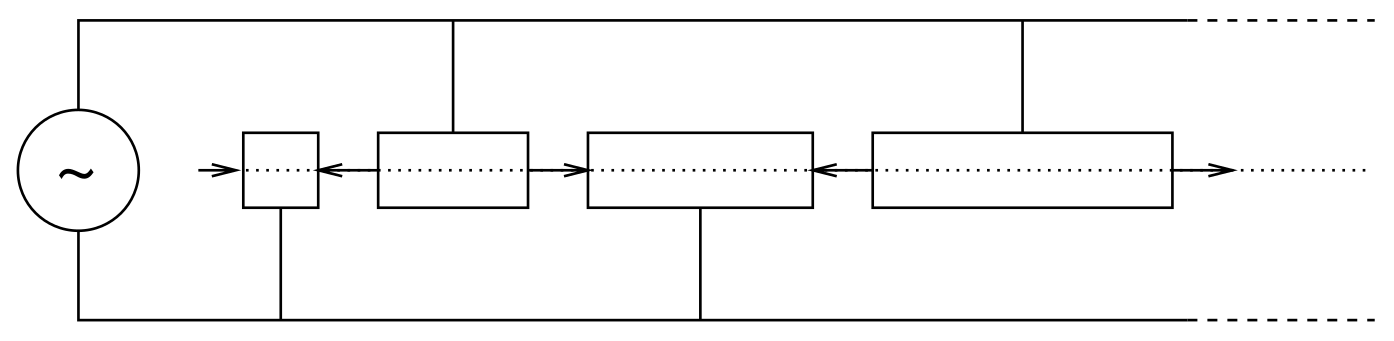
\includegraphics[width=0.5\textwidth]{Figures/Wideroe_Linac.png}
\caption[Schematic layout of a Wider\o e linac]{Schematic layout of a linear accelerator with drift chambers of increasing lengths after the design by Rolf Wider\o e.~\cite[p. 40]{Hinterberger}}
\label{fig:Wideroe_Linac}
\end{figure}
\\Nowadays, particle accelerators all over the world mainly use RF cavities instead of drift tubes, with the possibility of being made of superconducting material since the electric resistance is minimal due to their superconducting nature.
Unlike before the acceleration takes place inside the cavities, and all cavities are of the same length and shape.
Their characteristic shape has the effect that the electromagnetic (EM) wave inside the cavity is resonant.
Figure~\ref{fig:Tesla_Cavity} shows a 9-cell niobium cavity developed at Deutsches Elektronen-Synchrotron (DESY) in Hamburg besides other facilities.
Its shape is called ``TESLA-style'', and its accelerating gradient exceeds \SI{35}{\mega\volt\per\meter} whilst it can be tuned to a RF frequency of \SI{1.3}{\giga\hertz} .~\cite[p. 15f]{TDR31}
\begin{figure}
\begin{subfigure}[b]{0.49\textwidth}
\centering
 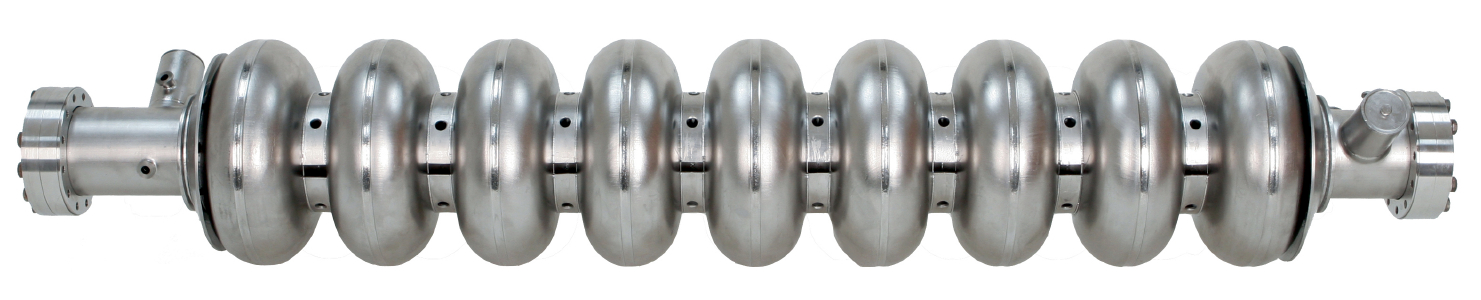
\includegraphics[width=\textwidth]{Figures/Tesla_Cavity.jpg}
\caption[Tesla-style 9-cell cavity]{Picture of a so-called TESLA-style 9-cell niobium cavity.~\cite[p. 15]{TDR31}}
\label{fig:Tesla_Cavity}
\end{subfigure}\hfill
\begin{subfigure}[b]{0.49\textwidth}
\centering
 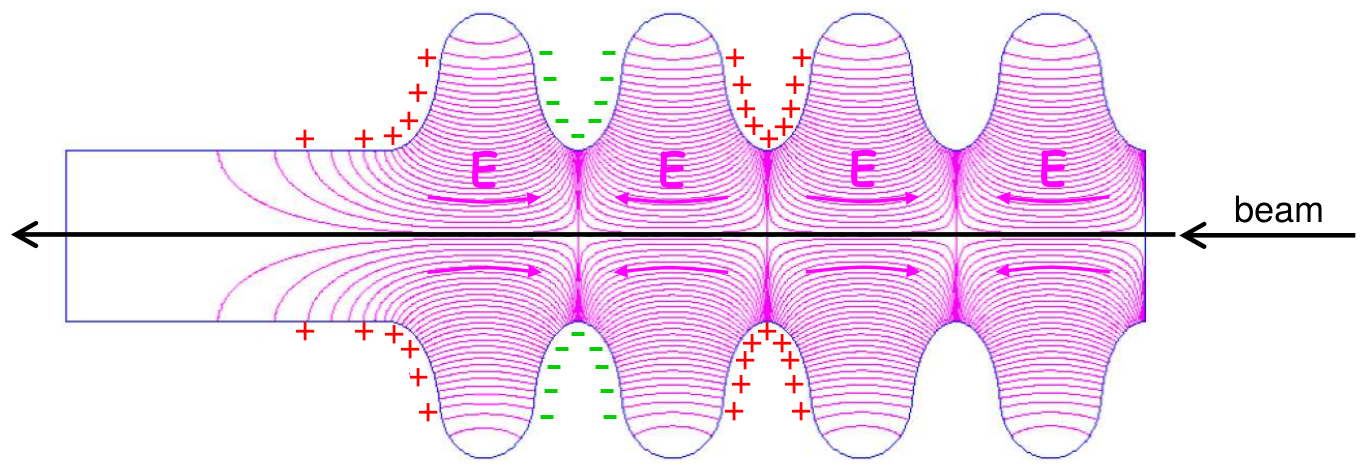
\includegraphics[width=0.9\textwidth]{Figures/Cavity.png}
\caption[Electric field in a cell cavity]{Schematic drawing of the electric field lines inside a cell cavity.~\cite[p. 47]{Desy_SummerStudent_Lecture}}
\label{fig:Cavity}
\end{subfigure}
\caption[RF cavities]{The multi-cell RF cavities have a characteristic shape which is modeled in such a way that the electromagnetic (EM) RF field inside the cavities become resonant. Figure (a) shows a 9-cell cavity with the ``TESLA'' shape. Figure (b) illustrates the field vectors of the EM field in the single cells of the cavity.}
\label{fig:Cavities}
\end{figure}
The RF field direction inside a cell is oscillating with the RF frequency, and neighboring cavity cells show opposite field directions (see Figure~\ref{fig:Cavity}).
The frequency is then tuned such that the beam always experiences an accelerating RF phase. 
Due to the nature of these accelerating structures, the beam has to be bunched in order to provide acceleration to all beam particles.
This bunching happens naturally:
With the particle momentum having a Gaussian distribution, slow particles, i.e. particles with smaller than the ideal momentum, arrive at the accelerating cavity later than the ideal particle, and faster particles earlier respectively.
Therefore particles will be accelerated by different phases of the RF field, as can be seen in Figure~\ref{fig:RFPhase}.
Particles arriving later will experience a higher phase and will be accelerated more, particles arriving too early will experience a smaller phase and therefore will be accelerated less.
The particles oscillate about the ideal stable phase, and therefore form beam bunches.
This oscillation is called ``synchrotron oscillation''.
\begin{figure}
\centering
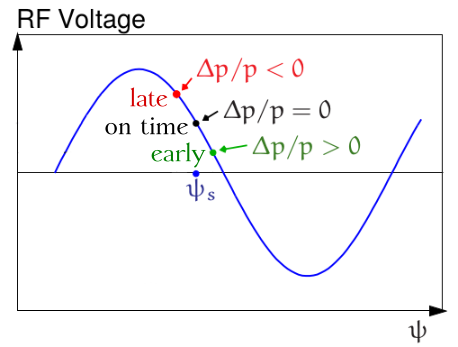
\includegraphics[width=0.4\textwidth]{Figures/RFphase.png}
\caption[Phase focusing]{RF voltage as a function of the RF phase. In the ideal case, the particles arrive at the RF phase $\psi_s$. 
Particles with a smaller momentum ($\Delta$p/p $<$ 0) will arrive later than the ideal particles, and will therefore be accelerated more, particles with larger momentum will be accelerated less respectively.}
\label{fig:RFPhase}
\end{figure}
%To still guarantee the particle to be accelerated by the same RF phase, the RF frequency is varied over the length of the linear collider.

Rolf Wider\o e did not only build the first linear accelerator, he even more importantly invented the principles of the betatron, the very first accelerating structure using electromagnetic fields.
Also the cyclotron which was invented in 1928 uses a magnetic field to deflect the charged particles on a radial path, and therefore allow the accelerator to be much smaller than before.
Exactly that idea was needed to advance from purely linear to circular in particle accelerators.

\subsection{Transversal beam dynamics}
\label{AccPhysics:Magnets}

Circular acceleration does also have certain challenges.
From the equilibrium of the Lorentz and the centripetal force follows:
\begin{align}
q(\vec{v}\times \vec{B}) &= \frac{m\vec{v}^2}{r}\\
qvB\vec{e_r} &= \frac{mv^2}{r}\vec{e_r} \nonumber \\
 r&=\frac{mv}{qB}\\
 &=\frac{p}{qB}\label{eq:MagField_Radius}
\end{align}
Since the momentum $p$ of the charged particle rises over time, the radius $r$ of its circular path increases if the magnetic field $B$ is constant.
The accelerator hence has to be built accordingly taking the increase in the radius into account, or needs to use magnets with variable field strengths.
Ladder is done in synchrotron machines, a type of circular accelerator combining the principles of all particle accelerators mentioned above: acceleration in RF cavities, variation of the RF frequency, and variable magnetic field strengths.
In this way, the particles are traveling along a stationary orbit, passing through the same magnets and cavities over and over again until the desired collision energy is reached.
To insure the stability of the orbit, not only bending dipole magnets can be found but also quadrupole magnets for focusing the particles, and sextupole and octupole magnets which then correct orbit fluctuations.
The need for higher order correction magnets can be derived from the expansion of the magnetic field around the ideal path of the particle (x = 0):
\begin{alignat}{5}
 B_y(x) &= B_{y0} &&+ \frac{\partial B_y}{\partial x}x &&+ \frac{1}{2!}\frac{\partial^2 B_y}{\partial x^2}x^2 &&+ \frac{1}{3!}\frac{\partial^3 B_y}{\partial x^3}x^3 &+ ...\\
 \intertext{When multiplying with $\frac{q}{p}$:}
 \frac{q}{p}B_y(x) &= \frac{q}{p}B_{y0} &&+ \frac{q}{p}\frac{\partial B_y}{\partial x}x &&+  \frac{1}{2!}\frac{q}{p}\frac{\partial^2 B_y}{\partial x^2}x^2 &&+ \frac{1}{3!}\frac{q}{p}\frac{\partial^3 B_y}{\partial x^3}x^3 &+ ...\\
  &= \frac{1}{r} &&+ kx &&+ \frac{1}{2!}mx^2 &&+ \frac{1}{3!}ox^3 &+ ... \label{eq:field_components}\\
  &\rightarrow \textnormal{dipole} &&+ \textnormal{quadrupole} &&+ \textnormal{sextupole} &&+ \textnormal{octupole} &+ ...\nonumber
\end{alignat}
Equation~\ref{eq:field_components} shows directly the connection between the radius and the magnetic field in the dipole component (compare with Equation~\ref{eq:MagField_Radius}).
In the quadrupole, sextupole and octupole components, a factor for the magnet strength is introduced.
According to the Maxwell equation $\vec{\nabla}\cdot\vec{B} = \frac{\partial B_y}{\partial x} -\frac{\partial B_x}{\partial y} = 0$, the Lorentz force on a particle in a quadrupole magnet, has therefore to be written as (cf. \cite[p. 372]{VacuumElectronics}):
\begin{multicols}{2}
\noindent 
\begin{align}
 F_x &= -qv\frac{\partial B_x}{\partial y}x \nonumber\\
  &= -q\beta c\frac{\partial B_x}{\partial y}x\\
  &= -gx\label{eq:Quad_Lorentz_x}
\end{align}
\columnbreak
\begin{align}
 F_y &= qv\frac{\partial B_y}{\partial x}y\nonumber \\
  &= q\beta c\frac{\partial B_y}{\partial x}y\\
  &= gy \label{eq:Quad_Lorentz_y}
\end{align}
\end{multicols}
From Equations~\ref{eq:Quad_Lorentz_x} and \ref{eq:Quad_Lorentz_y}, it becomes clear that quadrupoles can only focus in one direction, whilst it defocuses in the other.
A schematic cross-section of a quadrupole magnet is shown in Figure~\ref{fig:Quadrupole}, in which a positively charged particle would be focused in the y-direction and defocused in the x-direction.
The magnetic field lines point from the magnetic north pole to the south pole, and get denser towards the edges of the beam pipe.
The further a beam particle is away from the center, the stronger is the magnetic field it experiences, and the more it is deflected towards the center.
\begin{figure}
\centering
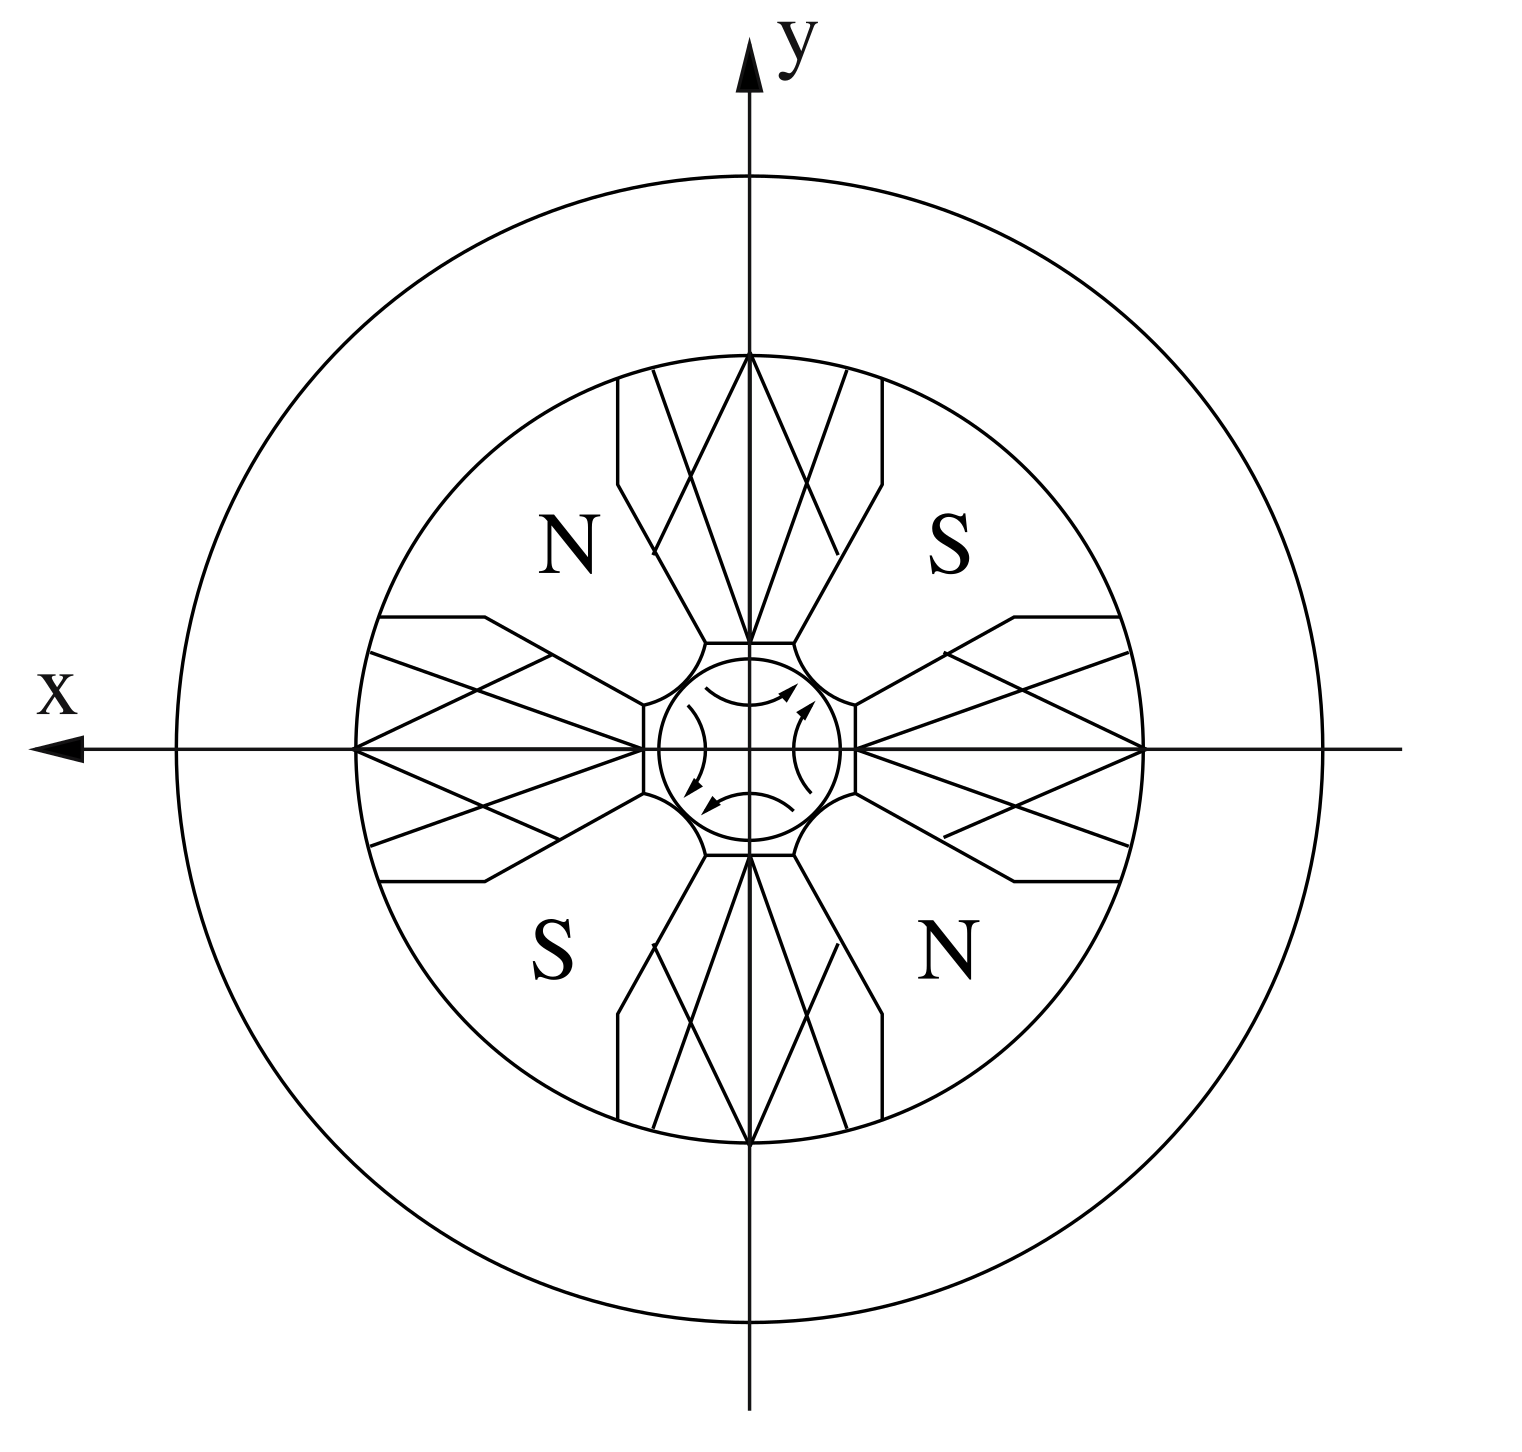
\includegraphics[width=0.4\textwidth]{Figures/Quadrupole.png}
\caption[Cross-section of a quadrupole magnet]{Schematic cross-section of a quadrupole magnet with the four magnetic north and south poles.
The beam pipe is centered in the middle between the pole shoes.
A positively charged particle inside the beam pipe would be focused in the y-direction and defocused in x.~\cite[p. 88]{Hinterberger}}
\label{fig:Quadrupole}
\end{figure}
\\Due to the fact that there are focusing and defocusing quadrupoles, so-called FODO structures are commonly used in particle colliders.
FODO is an alternating structure made out of focusing quadrupole magnets (``F'') and defocusing ones (``D''), with drift paths in between (see Figure~\ref{fig:FODO}).
After several of these structures, which act like optical lenses, the particle beam is focused in both directions, horizontally and vertically.
\begin{figure}
\centering
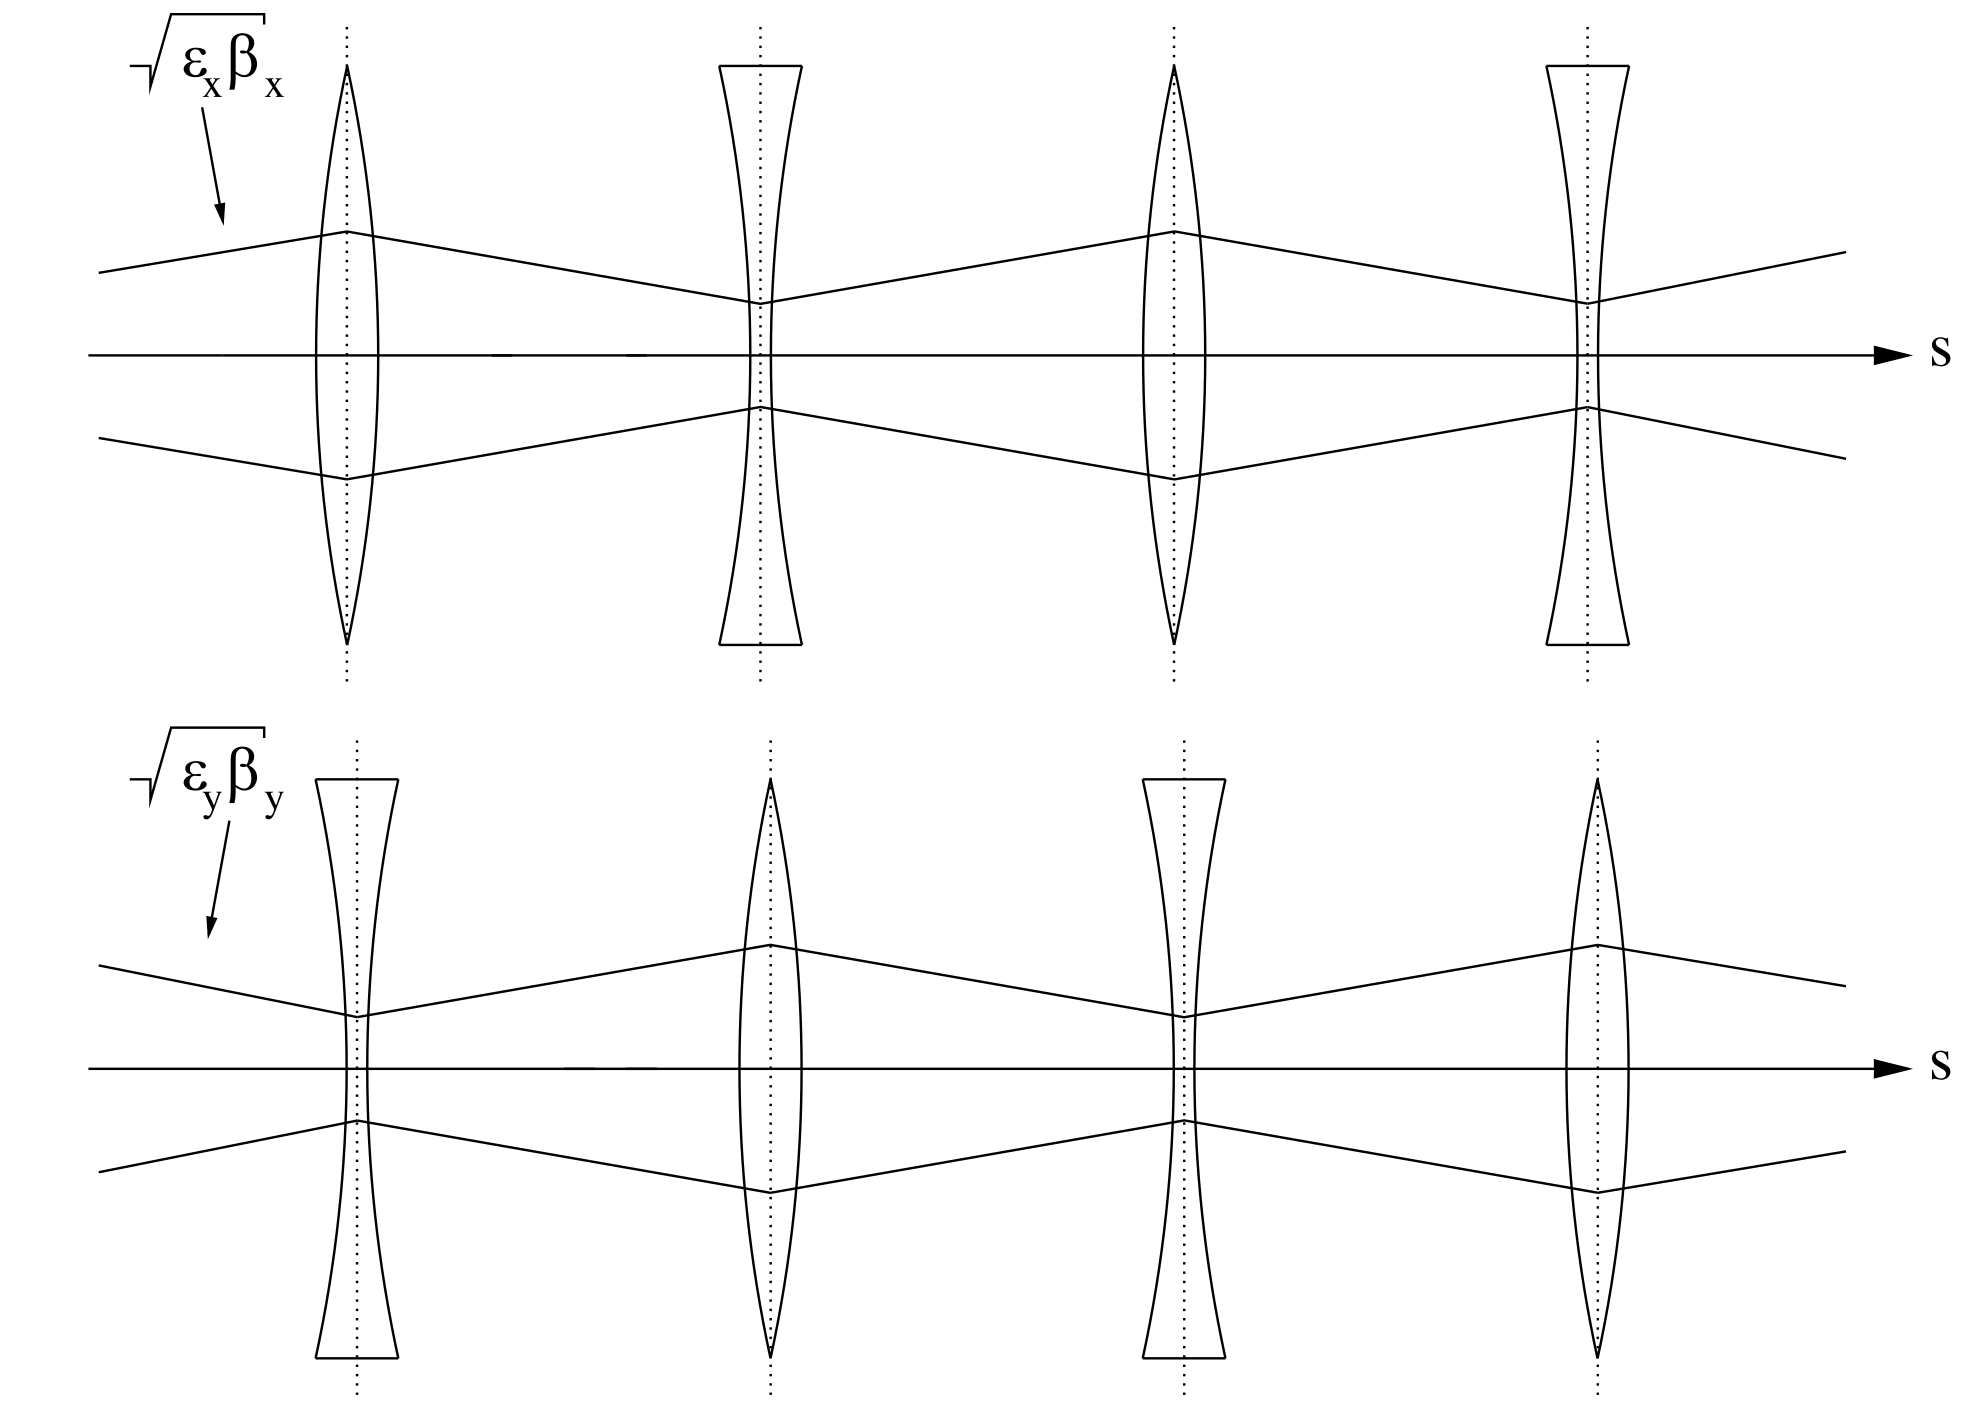
\includegraphics[width=0.5\textwidth]{Figures/FODO.png}
\caption[Schematic of FODO structure]{Schematic of a FODO structure in the horizontal and vertical plane. The particles are focused and defocused by the quadrupoles that act as lenses. The overall beam envelope is compressed after a certain number of focusing and defocussing quadrupoles.~\cite[p. 65]{Hinterberger}}
\label{fig:FODO}
\end{figure}
Due to the restoring force, particles that were deflected by the focusing magnets start to perform betatron oscillations around the ideal particle path.
The amplitude of these oscillations is the beam envelope that covers the paths of all beam particles, i.e. the maximum transverse beam dimension at a given location.
It can be expressed by the two beam parameters $\beta$ and $\epsilon$ which will be explained in the following:\\
The beta function $\beta$ describes the spatial dependency of the amplitude and the wave length of the betatron oscillations.
It is a periodic function, dependent on the focusing strengths and the order of the magnets in the beam line.
At any given point along the beam line, the $\beta$ value can be given in its units of length.
Of particular interest is its value at the interaction point (IP), the point of the beam collisions, where it is then  named $\beta^*$ .
The smaller the beta function is, the narrower is the beam.\\
Like the beta function, the transverse emittance $\epsilon$ is defined in the horizontal and vertical plane.
$\epsilon$ is a direct measure of the convergence of the beam with respect to its spread in space and in momentum.
A small emittance therefore means that the beam particles are confined to a small space, whilst they are all of the same momentum.
It also has the units of length, and is often given as the normalized emittance $\epsilon^* = \epsilon\gamma$, with the relativistic Lorentz factor $\gamma=\frac{1}{\sqrt{1-v^2/c^2}}$.\\
Together, the spatial amplitude of the betatron oscillations can be written as $A = \sqrt{\epsilon\beta}$.
Since the amplitude of these oscillations counts towards the size of the beam, it can then be written as $\sigma_{betatron} = A = \sqrt{\epsilon\beta}$.
The amplitude is also shown as the maximum extent in x in the so-called phase space ellipse, shown in Figure~\ref{fig:PhaseSpaceEllipse}.
The phase space consists of x and x', meaning the position and the momentum of the particles.
The ellipse drawn in the phase space is the region in which the motion of the particles is stable, it illustrates the qualities of the particle beam.
Since the particle's spread in position and momentum varies along the beam line, the shape of the ellipse changes constantly, but the area of the ellipse stays the same.
The variables $\alpha$ and $\gamma$ are defined here as: $\alpha = -\frac12\beta'$ and $\gamma = \frac{1+\alpha^2}{\beta}$.~\cite[]{Wiedemann}
\todo{Check reference to the phase space ellipse variables}
\begin{figure}[h]
\centering
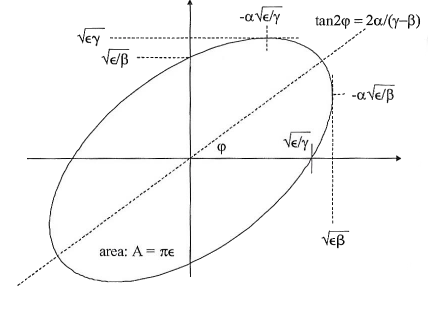
\includegraphics[width=0.5\textwidth]{Figures/PhaseSpaceEllipse.png}
\caption[Phase space ellipse]{Phase space ellipse~\cite[p. 158]{Wiedemann}}
\label{fig:PhaseSpaceEllipse}
\end{figure}
\todo{Exchange picture of phase space ellipse}
\\The actual transverse size of the beam is not yet fully defined by the spatial amplitude of the betatron oscillations.~\cite[cf. p. 108ff]{Conte}
Also the deviation from the ideal particle trajectory due to the momentum spread has to be taken into account, which is defined by the dispersion function $\eta$.
Like $\epsilon$ and $\beta$, it is dependent on the position along the beam line, and can be defined as $\eta = \frac{dx}{d\delta}$, with the fractional deviation from the ideal particle momentum $\delta = \Delta x'/x'_0$.
With this knowledge, the overall beam size can now be calculated:
\begin{align}
 \sigma&=\sqrt{\sigma^2_{betatron}+\sigma^2_{dispersion}}\\
 &=\sqrt{\epsilon\cdot\beta+\left(\eta\frac{\Delta x'}{x'_0}\right)^2}
\end{align}


\subsection{Linear colliders in comparison to circular colliders}
\label{Linear-Circular}
These transversal beam dynamics described in the section above are of course valid for circular as well as linear accelerators.
In both machines, the acceleration with RF cavities, for instance, is accompanied by beam deflections and corrections with the help of magnets.
Naturally, the beam line of a circular collider contains on average more magnets than a linear collider.\\
Currently, the world's largest circular particle collider is the Large Hadron Collider (LHC) at CERN in Switzerland, a synchrotron machine with a circumference of \SI{27}{\kilo\meter}.
The collision energy of the two colliding proton beams is \SI{13}{\TeV}, and its nominal peak luminosity \lumi is \SI{e34}{\centi\meter^{-2}\second^{-1}}.
The luminosity of a particle collider is proportional to the amount of collisions that can occur, and it is defined as:
\begin{align}
 \mathcal{L}&=\frac{N_1N_2 \cdot n_b \cdot f}{2\pi \cdot \sqrt{\sigma^2_{x,1}+\sigma^2_{x,2}} \sqrt{\sigma^2_{y,1}+\sigma^2_{y,2}}}\\
 \intertext{If the bunch sizes of the opposite beams are the same:}
 &=\frac{N_1N_2 \cdot n_b \cdot f}{4\pi \cdot \sigma_x \sigma_y}
\end{align}
$N_{1,2}$ is the number of particles per bunch, which is usually the same for both beams, so that $N_1=N_2$.
$f$ is the revolution frequency, the number of revolutions a bunch makes per second.
$n_{b}$ is the number of bunches, and $\sigma_{x,y}$ is the beam bunch size in the horizontal and the vertical plane.
Table~\ref{tab:ILC_parameters} in Chapter~\ref{ILC} lists these parameters and their values for the LHC in comparison to the International Linear Collider (ILC).
In order to translate the luminosity in an event rate, the luminosity value has to be divided by the cross-section $\sigma_p$ of the physics process that is of interest.
Since the LHC detectors do only measure events from inelastic scattering, the LHC event rate can be calculated by taking only the cross-section for inelastic proton-proton scattering into account, which is measured to be \SI{78}{\milli\barn}~\cite{inelXSection}.
\begin{align}
 \dot{N}&=\mathcal{L}\cdot\sigma_{inelastic}\\
 &=10^{34} \textrm{cm}^{-2}s^{-1} \cdot 78\textrm{\,mb}\\
 &=7.8\times 10^8 s^{-1}
\end{align}
%https://www.lhc-closer.es/taking_a_closer_look_at_lhc/0.cross_section
Per second about 780 million events are occurring at the LHC.
%The reason why large synchrotron rings need pre-accelerators is that the range for changing the magnet's field strength is limited.
The LHC is a so-called ``discovery machine''.
With its high luminosity and high collision energy, the possible physics processes from the hadron collisions cover wide energy ranges.  
New particles, first seen for example as resonance peaks in the measured mass spectra, can be discovered easier due to the large phase-space.
This was the case in 2012 for instance, when the LHC found a peak at an energy of \SI{126}{\GeV}, shortly after recognized as the very first measurement of a Higgs boson.~\cite{Higgs}

Why these so-called ``discovery machines'' are hadron and not lepton colliders, and why they are circular and not linear, is to be explained with the physical qualities of the colliding particles.
Hadrons are by definition composite particles, providing the possibility of covering a large energy range when during collision their partons are interacting.
This so-called deep inelastic scattering is explained in more detail in Chapter~\ref{StandardModel}.
In contrast to that, collision of leptons as elementary particles is the interaction of exactly these leptons at exactly their given energy.
This is one of the reasons why lepton colliders are called ``precision machines''.